\documentclass[]{emulateapj}
\usepackage{amsmath}

\usepackage[breaklinks,colorlinks,citecolor=blue,linkcolor=blue]{hyperref}
\usepackage{etoolbox}

\makeatletter

% Patch case where name and year are separated by aysep
\patchcmd{\NAT@citex}
  {\@citea\NAT@hyper@{%
     \NAT@nmfmt{\NAT@nm}%
     \hyper@natlinkbreak{\NAT@aysep\NAT@spacechar}{\@citeb\@extra@b@citeb}%
     \NAT@date}}
  {\@citea\NAT@nmfmt{\NAT@nm}%
   \NAT@aysep\NAT@spacechar\NAT@hyper@{\NAT@date}}{}{}

% Patch case where name and year are separated by opening bracket
\patchcmd{\NAT@citex}
  {\@citea\NAT@hyper@{%
     \NAT@nmfmt{\NAT@nm}%
     \hyper@natlinkbreak{\NAT@spacechar\NAT@@open\if*#1*\else#1\NAT@spacechar\fi}%
       {\@citeb\@extra@b@citeb}%
     \NAT@date}}
  {\@citea\NAT@nmfmt{\NAT@nm}%
   \NAT@spacechar\NAT@@open\if*#1*\else#1\NAT@spacechar\fi\NAT@hyper@{\NAT@date}}
  {}{}
  
\makeatother
%
\usepackage{xspace}
%
\usepackage{apjfonts}
\usepackage{amssymb, amsmath} % for e.g. \lesssim
\usepackage{natbibspacing, natbib}
\usepackage{aas_macros} % for understanding Journal in bib
\usepackage{graphics,graphicx}
%
\newcommand{\vdag}{(v)^\dagger}
\newcommand{\myemail}{tleung@astro.cornell.edu}
\newcommand{\Msun}{\mbox{$M_{\odot}$}\xspace}
\newcommand{\Rsun}{\mbox{$R_{\odot}$}\xspace}
\newcommand{\Lsun}{\mbox{$L_{\odot}$}\xspace}
\newcommand{\LIR}{\mbox{$L_{\rm IR}$}\xspace}
\newcommand{\LFIR}{\mbox{$L_{\rm FIR}$}\xspace}
%
\newcommand{\rarr}{$\rightarrow$}
\newcommand{\aco}{\mbox{CO($J$\,=\,1\,\rarr\,0) }}
\newcommand{\bco}{\mbox{CO($J$\,=\,2\,\rarr\,1) }}
\newcommand{\cco}{\mbox{CO($J$\,=\,3\,\rarr\,2) }}
\newcommand{\rot}[3][CO]{\mbox{#1($J$\,=\,#2\,\rarr\,#3)}}
%
\newcommand{\cii}{[C{\scriptsize II}]}
\newcommand{\Lp}[1][CO]{\mbox{$L^{\prime}_\textrm{\fontsize{8pt}{12pt}\selectfont{#1}}$}\xspace}
\newcommand{\kms}{\mbox{km\,s$^{-1}$}\xspace}
\newcommand{\LpU}{\mbox{K\,\,km\,\,s$^{-1}$\,\,pc$^2$}\xspace}
\newcommand{\pmOne}{\mbox{$^{-1}$}\xspace}
\newcommand{\alphaco}{\mbox{$\alpha_{\rm CO}$}\xspace}
\newcommand{\alphaU}{\mbox{$($K\,\,\kms\,\,pc$^2$$)$\pmOne}}
\newcommand{\sfrU}{\mbox{\Msun\,yr$^{-1}$}\xspace}
% Numerical values
\newcommand{\E}[1]{\mbox{$\times10^{#1}$}}
\newcommand{\petm}[2]{$^{+#1}_{-#2}$}
\newcommand{\eq}{\,=\,}
\newcommand{\pmm}{\,$\pm$\,}
%
\newcommand{\eg}{{e.g.,~}}
\newcommand{\ie}{{i.e.,~}}
%
\newcommand{\Fig}[1]{Figure~\ref{fig:#1}}
\newcommand{\Eq}[1]{Equation~\ref{eq:#1}}
\newcommand{\Tab}[1]{Table~\ref{tab:#1}}
\newcommand{\Sec}[1]{\S\ref{sec:#1}}
%
\newcommand\tna{\,\tablenotemark{a}}
\newcommand\tnb{\,\tablenotemark{b}}
\newcommand\tnc{\,\tablenotemark{c}}
\newcommand\tnd{\,\tablenotemark{d}}
\newcommand\tne{\,\tablenotemark{e}}
\newcommand\tnf{\,\tablenotemark{f}}
\newcommand\tng{\,\tablenotemark{g}}
\newcommand\tnh{\,\tablenotemark{h}}
\newcommand\tni{\,\tablenotemark{i}}
\newcommand\tnj{\,\tablenotemark{j}}
\newcommand\tnk{\,\tablenotemark{k}}
\newcommand\tnl{\,\tablenotemark{l}}
%
\def\herschel {{\it Herschel Space Observatory}\xspace}
\def\alma     {Atacama Large (sub-)Millimeter Array (ALMA)\xspace}
\def\spitzer {{\it Spitzer Space Telescope}\xspace}
\def\pdbi     {Plateau de Bure Interferometer\xspace}
\def\carma    {Combined Array for Research in Millimeter-wave Astronomy\xspace}
\def\cso      {Caltech Sumillimeter Observatory (CSO)\xspace}
\def\noema    {Northern Extended Millimeter Array (NOEMA)\xspace}
\def\vla      {{\it Karl G. Jansky} Very Large Array\xspace}
% Typography
\newcommand{\ncode}[1]{{\sc #1}}
% Codes / Softwares
\newcommand{\uvmcmcfit}{\ncode{uvmcmcfit}\xspace}
\def\aips {\ncode{AIPS}\xspace}
\def\casa {\ncode{CASA}\xspace}
% Long words
\newcommand{\lowZ}{low-metallicity\xspace}
\newcommand{\mulw}{multi-wavelength\xspace}
\newcommand{\SF}{star formation\xspace}
\newcommand{\SB}{starburst\xspace}
\newcommand{\SBs}{starbursts\xspace}
\newcommand{\gl}{gravitationally lensed\xspace}
\newcommand{\MCMC}{Markov Chain Monte Carlo (MCMC)\xspace}
% Wavelength regimes
\newcommand{\fir}{far-IR\xspace}
\newcommand{\fuv}{far-UV\xspace}
\newcommand{\mir}{mid-IR\xspace}
\newcommand{\nir}{near-IR\xspace}
\slugcomment{To be submitted to the ApJ}

\citestyle{aa}
\shorttitle{Something goes here}
\shortauthors{Leung \& Riechers}

\begin{document}
%{\tiny  \RevisionInfo}

\title{Molecular Gas Dynamics of the lensed wet-merger RXSJ1131-1123 at $z$=0.654}
\author{T. K. Daisy Leung and Dominik A. Riechers}
\affil{Department of Astronomy, Space Sciences Building, Cornell University,
Ithaca, NY 14853, USA; \myemail}
%==============================================================================
%                                Front matters
%==============================================================================

\begin{abstract}
\end{abstract}

\keywords{ISM: molecular --
          infrared: galaxies --
          galaxies: starburst --
          galaxies: evolution}

%--------------------------------------------------------------------------
%                                Introduction
%--------------------------------------------------------------------------
\section{Introduction}

%--------------------------------------------------------------------------
%                          Observations details
%--------------------------------------------------------------------------
\section{Observations}
\subsection{PdBI \bco} % DONE
Observations of the \bco rotational line ($\nu_{\rm rest}$ = 230.5379938 GHz)
toward the \gl galaxy RXJ1131-1231 at $z_{\rm QSO}$ =
0.658 were carried out using IRAM \pdbi (PdBI; Program ID: S14BX001; PI: D.
Riechers). Two observing runs were carried out on 2014 December 06 and 2015
February 05 under good weather conditions in the C and D array configurations,
respectively. The 2 mm receivers were used to cover the redshifted \bco line
and the underlying continuum emission, employing a correlator setup providing
an effective bandwidth of 3.6 GHz and a spectral resolution of 10.0 MHz ($\sim$
21.5 \kms). This resulted in 3.75 hours of cumulative six antenna-equivalent on-source
 time after discarding unusable visibility data.
The nearby quasars 1127$-$145 and 1124$-$186 were observed every 22 minutes
for pointing, secondary amplitude, and phase calibration and 1055$+$018 was
observed as bandpass calibrators for both tracks.
MWC349 and 3C279 were observed as the primary flux calibrator for C and D
array observations, respectively, yielding $\lesssim$15\% calibration accuracy.

The \ncode{GILDAS} package was used to reduce and analyze the visibility data
which are then imaged and deconvolved using the CLEAN algorithm with ``natural"
weighting. This yields a synthesized clean beam size of 4$\farcs$44 $\times$ 1\farcs95 (PA = 13\degr).
The final rms noise is $\sigma$ = 1.451 mJy \kms
beam\pmOne over 10 MHz (21.5 \kms). The continuum image at $\nu_{\rm cont}\sim$
139 GHz is created by averaging over all the line-free channels. This
yields an rms noise of 0.082 mJy beam$^{-1}$. % see README.md in 04Sep15

\subsection{CARMA \cco} %DONE
Observations of the \cco rotational line ($\nu_{\rm rest}$ = 345.7959899 GHz)
were carried out under the D array configurations of the \carma (CARMA;
Program ID: cf0098; PI: D. Riechers) on 2014 February 02 under terrible 1.5\,mm
weather conditions and on 2014 February 17 under good 1.5\,mm
weather conditions. The correlator setup provides a bandwidth of 3.75 GHz in
each sideband and a spectral resolution of 12.5 MHz ($\sim$17.9 \kms). The
line was placed in the lower sideband with the local oscillator tuned to $\nu_{\rm LO}\sim$216 GHz. The radio quasars J1127$-$189 (first track) and 3C273
(second track) were observed
every 15 minutes for pointing, amplitude, and phase calibration. Mars was
observed as the primary absolute flux calibrator and 3C279 was observed as
bandpass calibrators for both tracks. This results in a total on-source time of 2.94 hours after flagging poor
visibility data.

% poor phase note
% /Users/admin/Research/RXJ1131/CARMA/imagingD23/checkQuality.csh
%
% calflux source=1127-189 in=$MIRCAT/FluxSource.cat device=/xs
% Flux of: 1127-189  14FEB04.50 at 227.0 GHz:  0.65 Jy; rms: 0.10 Jy
% Extrapolate to 215.673 GHz with spectral index = -0.986 --> 0.684 Jy
% MIRIAD from bootstrap: Median Flux @ 215.673 GHz:     0.710
Given that the phase calibrator used for the first track was faint and was
observed under poor weather conditions and that the phase calibrator used for
the second track was far from our target source, the phase calibration is
subpar, with an rms scatter $\sim$60\degr. We thus conservatively estimate
a calibration accuracy of $\sim$45\% based on the flux scale uncertainties,
gain variation over time, and the phase scatter on the calibrated data. We
therefore treat its line intensity with caution and refrain using it to derive other physical quantities.

The \ncode{MIRIAD} package was used to calibrate the visibility data which are
then imaged and deconvolved using the CLEAN algorithm with ``natural" weighting. This yields a synthesized clean
beam size of 3\farcs2 $\times$ 1\farcs9 (PA = 8\degr) for the lower sideband
image cube. The final rms noise is $\sigma$ = 13.3 mJy km s$^{-1}$ beam$^{-1}$
over a channel width of 25 MHz. An rms noise of
$\sigma$ = 0.831 mJy beam\pmOne is reached by averaging over the
line-free channels.


\subsection{VLA} %DONE
Our analysis also use the archival data of the radio continuum obtained with the \vla (VLA; Program ID: AW741; PI: Wucknitz). Since these data have not been
published, we here describe the details of the observations as well as our calibration steps.

Observations were carried out on 2008 December 29 under excellent weather
conditions in the A array configurations for a total of $\sim$7 hours on-source time. The C$-$band receivers were used with a continuum mode setup,
providing a bandwidth of 50 MHz in each sideband.
The nearby radio quasar 1130$-$149 was observed every 10 minutes for
pointing, amplitude, and phase calibration, 1331$-$305 was observed as the
primary flux calibrator, and 0319$+$415 was observed as the bandpass
calibrator, yielding $\sim$10\% calibration accuracy.
We use \aips to calibrate the visibility data which
are then imaged and deconvolved using
the CLEAN algorithm using robust\,=\,0. This yields a synthesized clean
beam size of 0$\farcs$49 $\times$ 0\farcs35 (PA\,=\,0\farcs18) and a final
rms noise of $\sigma$ = 13 $\mu$Jy beam\pmOne.


\section{HST astrometry}
We obtain HST images from the Hubble Legacy Archive with
a goal to understand the origins of the emission detected
in our mm observations. We adopt the VLA 5\,GHz map of $\sim$0\farcs5
resolution as the reference coordinate frame to align the optical (V$-$band) image.
We shift the latter to the east by 0\farcs5963 in R.A. and $+$0\farcs8372 in
Dec., which is consistent with the typical astrometric precision (1$-$2") of
images from the Hubble Legacy Archive\footnote{http://hla.stsci.edu/hla\_faq.
html}. Such astrometric correction is critical to avoid artificial spatial
offsets between different emitting regions and to carry out our lens modeling,
in which the absolute position of the foreground lensing galaxy is guided by its
coordinates in the optical image, where its emission is clearly detected.
The VLA image is calibrated using a well-monitored phase
calibrator, with absolute positional accuracy of $\sim$2 mas.
For this reason, the absolute alignment between the VLA image and other
interferometric images reported in this paper are expected to have astrometric
precision better than 0\farcs1, modulo uncertainties related to the SNR, phase
errors, and beam size.

%--------------------------------------------------------------------------
%                                Results
%--------------------------------------------------------------------------
\section{Results}
\subsection{\bco Emission} %DONE
We dynamically resolved the \bco line emission toward the background galaxies
at $\gtrsim$27$\sigma$ significance, confirming the redshift at $z_{\rm CO}$ =
0.65370 $\pm$ 0.0005. A highly asymmetric double-horned line profile is
detected as shown in \Fig{CO21spec}. Fitting a double Gaussian results in peak
flux densities of 75.3$\pm$2.6 and 24.0$\pm$2.0 mJy, and a FWHM of
179$\pm$9 \kms and 255$\pm$28 \kms, respectively. The peaks are separated by
$\Delta v_{\rm sep}$ = 220 \kms. The integrated line flux is 24.1\,$\pm$\,2.3 Jy \kms. % see 15May16/

\begin{figure}[tbph]
\centering
\includegraphics[width=0.45\textwidth]{../Figures/SpecCO21_twinx.eps}
\caption{ Spectrum of \bco emission toward RXJ1131. The velocity scale
is with respect to $z$=0.6537, which is approximately the line center
considering the asymmetry is as a result of differential lensing.
A more detailed discussion of differential lensing effect is presented in
\Sect{differential} and the magnification factors for various kinematic
components are listed in \Tab{mag}.
 \label{fig:CO21spec}}
\end{figure}

% moment 0 map: CASA chan=125~159 <=> GILDAS 126-160 <=> python 125-160
% - sigma = 0.305 Jy km/s/Beam
%   - note that theoretical sigma is lower = 1.5 * sqrt(160-126+1) * 21.5 ~ 0.2 Jy km/s /beam, due to higher noise in some channels with emission
We construct the zeroth, first and second moment maps shown in \Fig{CO21mom}
using the $uv$-continuum subtracted data cube, over $\Delta v$$\sim$750 \kms.
The first and second moment maps are clipped at 3$\sigma$.
The peak flux density is 8.12 $\pm$ 0.30 Jy\,\kms\,beam\pmOne in the intensity-
integrated map. The deconvolved source size is estimated to be 5\farc1$\pm$0\farc72 $\times$ 3\farcs72$\pm$0\farcs66 and thus the emission is resolved over
$\sim$2.2 beams. While the lensed emission is not strictly distributed as 2D-
Gaussian, the fit recovers the line intensity enclosed within the emitting
region, we therefore take this as an estimate on the extent of the lensed
emission. On the other hand, if we assume the spatial distribution of
the lensed molecular gas emission is similar to that in the optical to \nir
wavelengths, the lensed emission would be more accurately described by an
annulus, including the partially complete ``Einstein Ring" and
the lensed knots (see \Fig{CO21mom)}.

\begin{figure}[!htbp]
\centering
\includegraphics[trim=0 5 0 15, clip, width=0.25\textwidth]{../Figures/{F555WCO21_mom0_single.invertedgray}.eps}
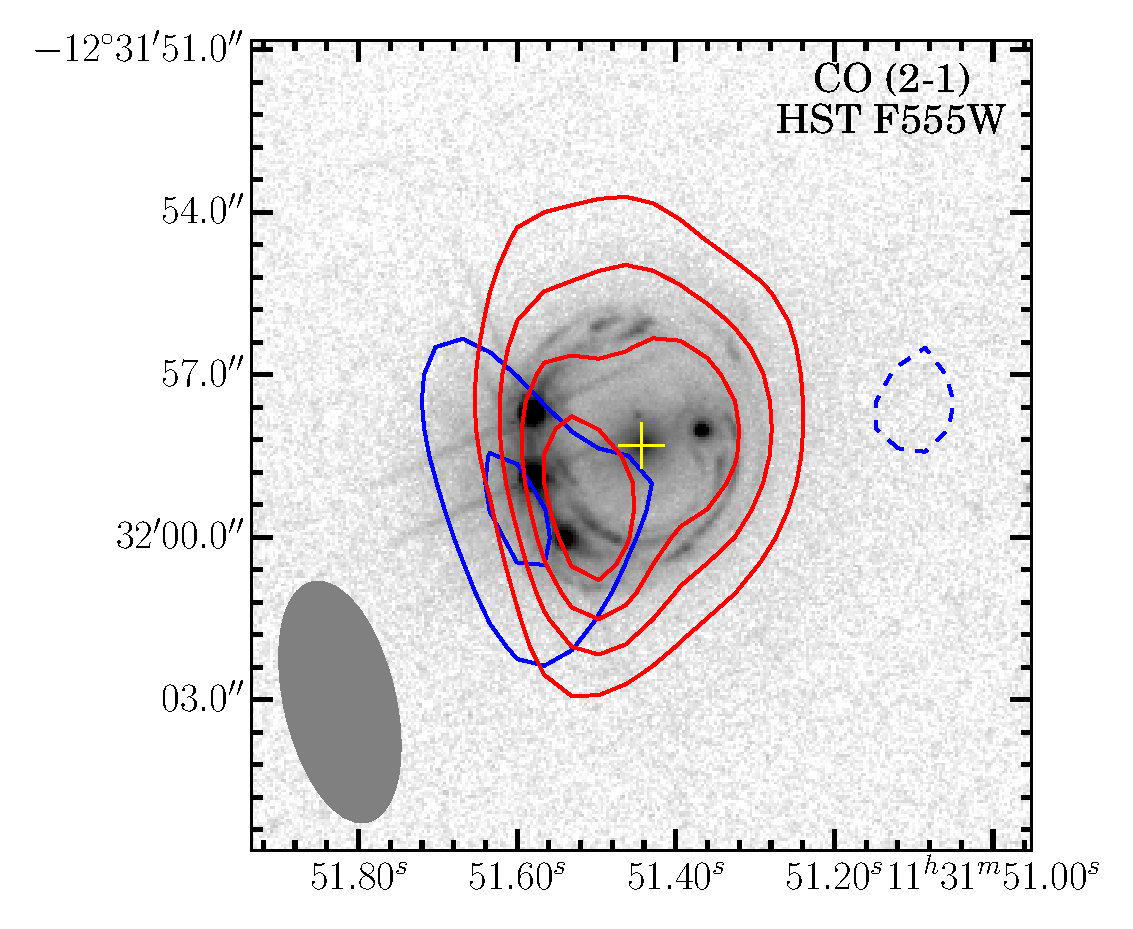
\includegraphics[trim=0 5 0 15, clip, width=0.25\textwidth]{../Figures/F555W_REDBLUE.eps}
\includegraphics[width=0.5\textwidth]{../Figures/CO_highOmom_CLIP5sigma}
\caption{
An overlay of the velocity-integrated \bco emission on the HST V$-$band (F555W)
image. The contours start at 3$\sigma$ and increment at steps of
$\pm$3$\sigma$, where $\sigma$=0.3 mJy beam\pmOne. The cross denotes the
location of the foreground galaxy at $z$=0.295. {\it Right: } The contours
are color coded to represent the red and blue wings of the emission.
\label{fig:CO21mom}}
\end{figure}

The emission of the red component coincides with the Einstein Ring seen in the
optical image, with most of its apparent flux originating from the lensed arc
in the Southeast, whereas the blue component is predominately coming from
solely the lensed arc shown in \Fig{CO21mom}. To illustrate this, we show the
channel maps of 21.5\,\kms width and spatial spectra of 1\farcs5 resolution in
\Fig{chanmap} and \Fig{spatial}, respectively. The figures show that emission
is present to the West and peaks toward the lensing arc (black across in \Fig{
chanmap}) in the red wing, and shifts to the East with decreasing velocity (
blue wing). This indicates extended emission in the source plane, where
emission from different kinematic components is separated by different amounts
relative to the caustics. One consequence of such is the observed asymmetric
line profile. A detailed analysis on differential lensing of \bco is presented in \Sec{differential}.

\begin{figure*}[!htbp]
\centering
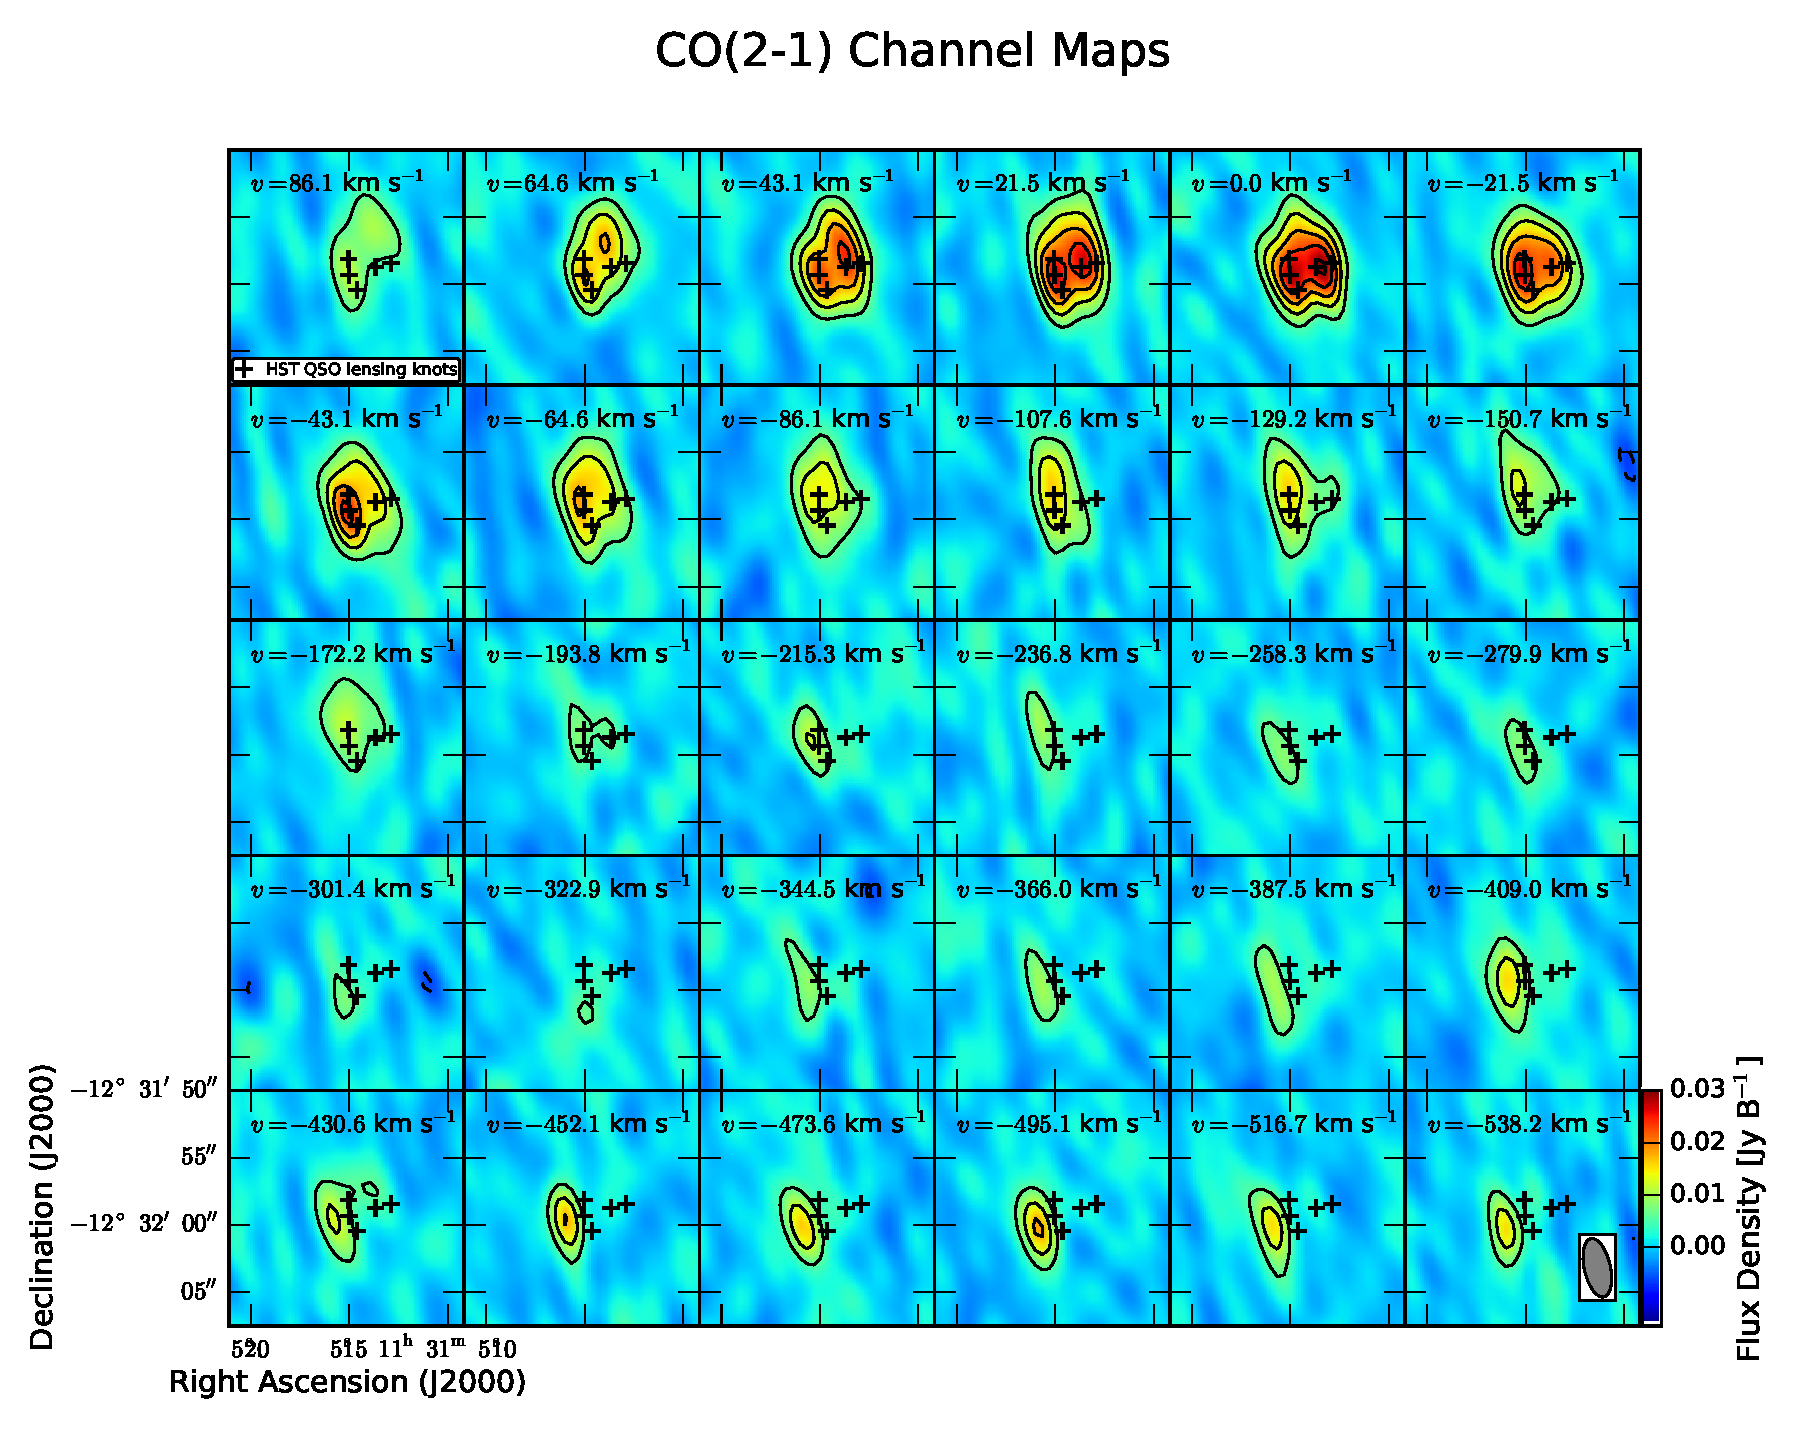
\includegraphics[width=0.9\textwidth]{../Figures/co_channel_maps.eps}
\caption{
Channel maps of \pdbi \bco toward RXJ1131 in 21.5\,\kms resolution. The
Black crosses indicate the position of the lensed knots (AGN emission,
which are components ABCD in C06). The central white-filled
star indicates the position of the foreground lensing galaxy (component G
in C06), as detected in the HST image. Contours start and increment at steps of
$\pm$3$\sigma$. The beam is denoted in the bottom right panel. \label{fig:chanmap}}
\end{figure*}

\begin{figure*}[!htbp]
\centering
\includegraphics[width=0.9\textwidth]{../Figures/spatialSpec_offsetShifted.eps}
\caption{
\bco spectrum as a function of position, binned by 3 pixels in each
direction (1\farcs5). The spectra map covers an extent of $\sim$10"$\times$10"
centering on the pixel that corresponds to the lensing galaxy. The velocity
and flux density scales are denoted in the top right panel.
BLAH: DR would want the pixel coordinates replaced by arcsec offset from
center. \label{fig:spatialSpec}}
\end{figure*}

We place an upper limit on \rot[HNC]{2}{1} line emission at the red-shifted
frequency 140 GHz in the foreground galaxy at $z\sim$0.295) of
$\sigma$ = 1.451mJy per channel beam\pmOne.
Assuming a typical line width of 300 \kms, this corresponds to a 3$\sigma$
limit of 4.353 mJy \kms beam\pmOne.

\susbsection{Origin of the \bco emission} \label{sec:origin} %DONE
Evidently, the CO emission is co-spatial with the lensed optical emission in
the background AGN host galaxy. The question is then whether the optically
faint companion also contributes to the CO flux and thus contains a
non-negligible amount of molecular gas.
Indeed, based on our lens model presented in \Sec{lensmodel}, we find it
highly likely that part of the CO emission originates from
the companion. We thus classify RXJ1131 as a ``wet-wet'' merger.
However, we cannot quantify this with a mass ratio given the
spatial resolution. This will be verified in future higher-resolution observations. In the subsequent sections, we will interpret RXJ1131
using this scenario (i.e. a ``wet-wet'' merger).

\subsection{\bco Kinematics} % DONE
A clear velocity gradient and an unusually high
velocity dispersion ($\gtrsim$400\kms) near the central region
is seen in \Fig{CO21highO}. While beam smearing is inevitably the
dominant factor in the observed velocity dispersion
at the spatial resolution of this data, the exceedingly
high velocity dispersion hints
at potential perturbations from the AGN, or internal turbulence due to
interactions with the companion, and/or instability due to the large gas
content. A velocity gradient across the source plane in \Fig{model} is also
found in our lens model. This further supports the idea of a kinematically-
ordered galaxy, but its emission has been lensed differentially.
In this scenario, RXJ1131 is a disrupted disk galaxy hosting an optically
bright quasar and is in the process of merging.
We will defer the discussion of the implications to \Sec{dynamics},
where we analyze the dynamics of the system in the source plane.

\begin{figure}[!htbp]
\centering
\includegraphics[trim=0 5 0 15, clip, width=0.25\textwidth]{../Figures/{F555WCO21_mom0_single.invertedgray}.eps}
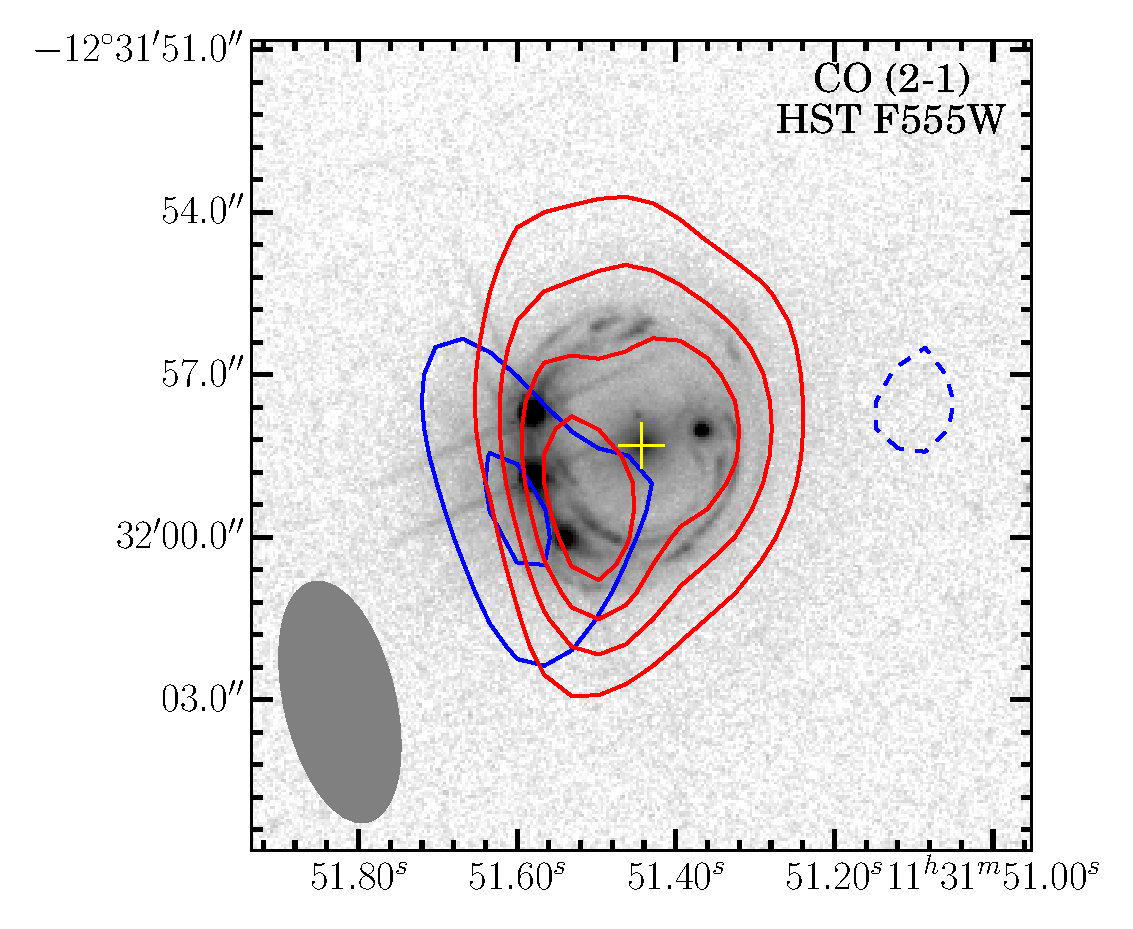
\includegraphics[trim=0 5 0 15, clip, width=0.25\textwidth]{../Figures/F555W_REDBLUE.eps}
\includegraphics[width=0.5\textwidth]{../Figures/CO_highOmom_CLIP5sigma}
\caption{
Contours for the first (left) and second (right) moment maps are shown in steps of 50 \kms, and 100 \kms, respectively. The beam (native resolution) is shown in the right panel.
\label{fig:CO21highO}}
\end{figure}


\subsection{\cco Emission} % DONE
We detect resolved \cco line emission toward RXJ1131. The spectrum is shown in
\Fig{co32spec}, which seems to have a double-peak profile.
This is expected if RXJ1131 is truly a disk galaxy (see previous
sections). The high phase noise in the calibration leads to a low SNR
detection. We thus estimate the line intensity to be
35.7$\pm$ 21.9 Jy\,\kms by summing up fluxes over the
linewidth used to infer \bco line intensity ($\sim$700 \kms).

\begin{figure}[!Htbp]
\centering
\includegraphics[width=0.5\textwidth]{../Figures/coOverlay.eps}
\caption{
\carma \cco line profile (solid) without continuum subtraction is
over-plotted on the continuum-subtracted \bco line profile (dashed).
The velocity scale is with respect to $z$=0.6537, which corresponds to the
dynamical center of the \bco line. The spectral resolution for \cco and \bco
is 35.8 \kms and 21.5 \kms, respectively.
 \label{fig:co32spec}}
\end{figure}

Assuming the spatial extents between \bco and \cco are similar and therefore
a negligible differential lensing effect, the line intensities
correspond to a brightness temperature ratio of
$r_{\rm 32}$\,=\,T$_{\tiny \cco}$/T$_{\tiny \bco}$\,=\,0.66$\pm$0.41.
The high uncertainty is dominated by the uncertainties in the \cco line
intensity.

\subsection{Interferometric Continuum} %DONE
No 1.5\,mm continuum emission is detected at the position of \cco
down to a 3$\sigma$ limit of 2.49mJy beam\pmOne.
This is consistent with the spectrum shown in \Fig{co32spec}.

We detect PdBI 2\,mm continuum in \Fig{2mm}. The integrated flux density is
1.2$\pm$0.2 mJy, with a peak flux $S_\nu$ = 800$\pm$88 \micron Jy\,beam\pmOne
centering on the lensing galaxy. A slightly extended emission is also seen
along the lensed arc. This suggests that the detected emission comes from
both the foreground galaxy and the background galaxy and that the
emission is marginally resolved along its major axis.
We subtract a point source model in $uv$-plane to remove the unresolved
emission toward the foreground galaxy. The peak flux (0.389$\pm$0.082 mJy)
in the residual map coincides with the lensed arc, and is consistent with
the difference between the integrated and the peak flux in the
original continuum map ($\sim$0.4 mJy). We therefore adopt
$S_\nu$ = 0.39$\pm$0.08 mJy as the 2\,mm continuum emission toward
the background galaxy.

\begin{figure}[!htbp]
\centering
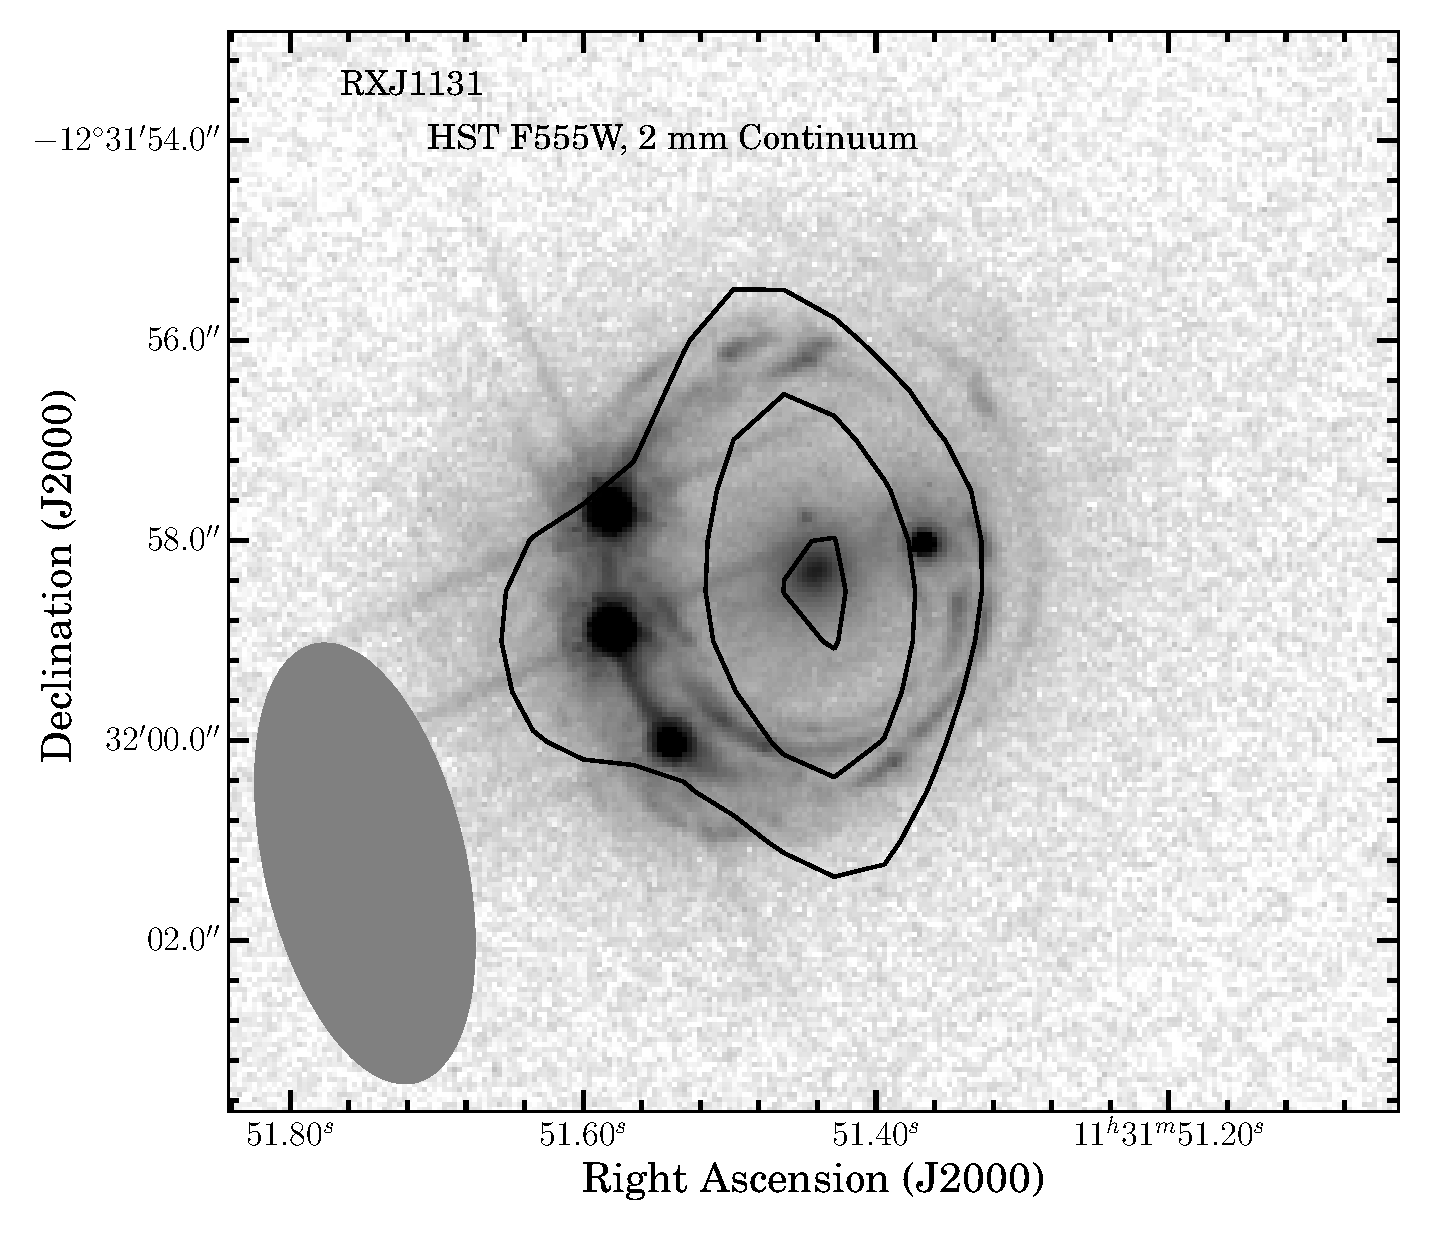
\includegraphics[width=0.35\textwidth]{../Figures/F555W_ContPdBI.eps}
\caption{
An overlay of the 2\,mm continuum emission on the optical image. Contours start and increment at steps of $\pm$3$\sigma$, where $\sigma$\,=\,0.082 mJy
beam\pmOne. The central cross indicates the centroid of the foreground galaxy,
as detected in the optical image. The synthesis beam is shown in the bottom left corner.
\label{fig:2mm}}
\end{figure}

\begin{figure}[!htbp]
\centering
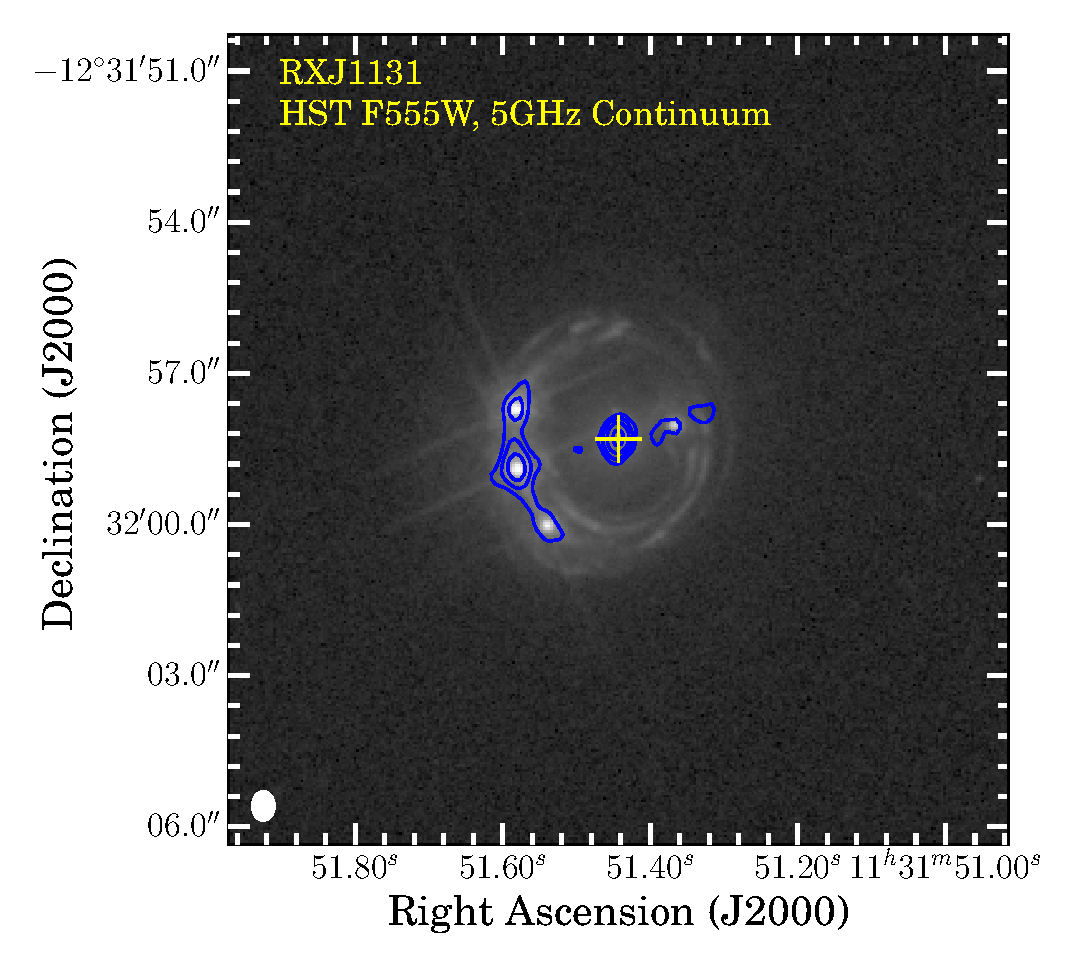
\includegraphics[width=0.35\textwidth]{../Figures/F555W_ContVLA.eps}
\caption{
VLA 5\,GHz continuum emission is overlaid on the optical image. Contours start and increment at steps of $\pm$3$\sigma$ of $\sigma$=13\micron Jy beam\pmOne. The beam is shown in the bottom left corner.
 \label{fig:vla}}
\end{figure}

The VLA C-band continuum image in \Fig{vla} shows resolved emission from the
jets and core of the foreground elliptical galaxy
as well as emission toward the background quasar.
Multiple peaks are seen along the arc and their centroids
coincide with the optical emission from the quasar.
We extract the flux densities for the arc and the core in \Tab{photometry}.
We find a spectral index of $\alpha$\,=\,0.024 for the foreground
galaxy and $\alpha$\,=\,0.345 for the background galaxy by fitting a
power-law (S$_\nu \propto \nu^{-\alpha}$) to the continuum emission at
5\,GHz and 2\,mm.


\subsection{Photometry}
We compiled/web-scraped the \mir to \fir photometry
from 2MASS, WISE, IRAS, IRAC catalogs .
to characterize
the dust emission in RXJ1131 from
from the 2MASS All-Sky Catalog of Point Sources  (Skrutskie et al. 2006), WISE
magnitudes from the AllWISE Source CatalogBLAH, Spitzer/MIPS
data from BLAH Catalog, IRAS photometry from the IRAS point source
and faint source cataloguesBLAH.

We extract the Herschel/SPIRE photometry using SUSSEXTractor
within HIPE (Savage \& Oliver 2007, Smith et al 2012, Pearson et al 2014)
over the data obtained from the Herschel Science Archive, which were
processed by the SPIRE HIPE pipeline version 12BLAH (Ott 2010).
The SUSSEXtractor
task estimates the flux density from an image smoothed with
a convolution kernel derived from the SPIRE beam FWHM.
The flux density measured by SUSSEXtractor
was verified using the SPIRE Timeline Fitter (Bendo et
al. 2013) which fits a two dimensional elliptical Gaussian
function at the source position in the timeline data. The
agreement between the SUSSEXtractor and Timeline Fitter
flux densities was found to be better than $\sim$BLAH per cent.

We list the photometry from optical to radio in \Tab{photometry}.
\begin{deluxetable}{lccc}[tbpH]
\tabletypesize{\scriptsize}
\tablecolumns{4}
\tablecaption{Photometry data}
\tablehead{\colhead{Wavelength } & \colhead{Frequency } & \colhead{Flux Density } & \colhead{Instrument}\\ \colhead{micron} & \colhead{GHz} & \colhead{mJy} & \colhead{ }}
\startdata
0.555 & 540167.0 & 0.056 $\pm$ 0.006 & HST-ACS/V-Band(L) \\
0.555 & 540167.0 & 0.009 $\pm$ 0.0041 & HST-ACS/V-Band(H) \\
0.814 & 368295.0 & 0.238 $\pm$ 0.013 & HST-ACS/I-Band(L) \\
0.814 & 368295.0 & 0.041 $\pm$ 0.0054 & HST-ACS/I-Band(H) \\
1.25 & 239834.0 & 1.009 $\pm$ 0.09 & 2MASS/J-Band \\
1.6 & 187370.0 & 0.539 $\pm$ 0.041 & HST-NICMOS(NIC2)/H-Band(L) \\
1.6 & 187370.0 & 0.133 $\pm$ 0.004 & HST-NICMOS(NIC2)/H-Band(H) \\
1.65 & 181692.0 & 1.448 $\pm$ 0.12 & 2MASS/H-Band \\
2.17 & 138153.0 & 2.064 $\pm$ 0.16 & 2MASS/Ks-Band \\
3.4 & 88174.2 & 7.027 $\pm$ 0.14 & WISE/W1 \\
3.6 & 83275.7 & 5.618 $\pm$ 0.0021 & Spitzer/IRAC(Extracted) \\
3.6 & 83275.7 & 5.034 $\pm$ 0.0021 & Spitzer/IRAC(Host) \\
3.6 & 83275.7 & 0.585 $\pm$ 0.003 & Spitzer/IRAC(Archive-Host) \\
4.5 & 66620.5 & 7.803 $\pm$ 0.0021 & Spitzer/IRAC(Archive) \\
4.5 & 66620.5 & 6.009 $\pm$ 0.0017 & Spitzer/IRAC(Host) \\
4.5 & 66620.5 & 1.794 $\pm$ 0.0027 & Spitzer/IRAC(Archive-Host) \\
4.6 & 65172.3 & 8.872 $\pm$ 0.16 & WISE/W2 \\
5.8 & 51688.4 & 10.720 $\pm$ 0.0051 & Spitzer/IRAC(Archive) \\
5.8 & 51688.4 & 7.557 $\pm$ 0.003 & Spitzer/IRAC(Host) \\
5.8 & 51688.4 & 3.163 $\pm$ 0.0059 & Spitzer/IRAC(Archive-Host) \\
8.0 & 37474.1 & 14.470 $\pm$ 0.0041 & Spitzer/IRAC(Archive) \\
8.0 & 37474.1 & 9.881 $\pm$ 0.0039 & Spitzer/IRAC(Host) \\
8.0 & 37474.1 & 4.589 $\pm$ 0.0057 & Spitzer/IRAC(Archive-Host) \\
12.0 & 24982.7 & 21.960 $\pm$ 0.42 & WISE/W3 \\
12.0 & 24982.7 & 400.000 $\pm$ \nodata & IRAS \\
22.0 & 13626.9 & 55.110 $\pm$ 1.9 & WISE/W4 \\
24.0 & 12491.4 & 47.180 $\pm$ 0.026 & Spitzer/MIPS \\
25.0 & 11991.7 & 500.000 $\pm$ \nodata & IRAS \\
60.0 & 4996.54 & 600.000 $\pm$ \nodata & IRAS \\
100.0 & 2997.92 & 1000.000 $\pm$ \nodata & IRAS \\
250.0 & 1199.17 & 289.427 $\pm$ 9.6 & Herschel/SPIRE \\
350.0 & 856.55 & 168.229 $\pm$ 8.6 & Herschel/SPIRE \\
500.0 & 599.585 & 56.782 $\pm$ 8.8 & Herschel/SPIRE \\
1387.93 & 216.0 & 2.492 $\pm$ \nodata & CARMA \\
2152.82 & 139.256 & 1.230 $\pm$ 0.22 & PdBI-integrated \\
2152.82 & 139.256 & 0.799 $\pm$ 0.082 & PdBI-peak \\
2152.82 & 139.256 & 0.400 $\pm$ 0.082 & PdBI-removedFG \\
61414.0 & 4.8815 & 1.273 $\pm$ 0.042 & VLA/Cband-arc \\
61414.0 & 4.8815 & 0.866 $\pm$ 0.027 & VLA/Cband-core
\enddata
\label{tab:BLAH}
\tablecomments{blah}
 %TablenotegoesBetween 
\tablerefs{blah}
\end{deluxetable}



%--------------------------------------------------------------------------
%                                Analysis
%--------------------------------------------------------------------------
\section{Analysis}
\subsection{Lens modeling} \label{lensmodel}
The spectrally resolved lensed emission allows us to probe dynamical structures on smaller spatial scales than otherwise possible.


With the high SNR and spectral resolution, we model different kinematic components using our lensing code \uvmcmcfit.

% describe model setup.


% comparison with C06 model


\begin{figure*}[tbph]
\centering
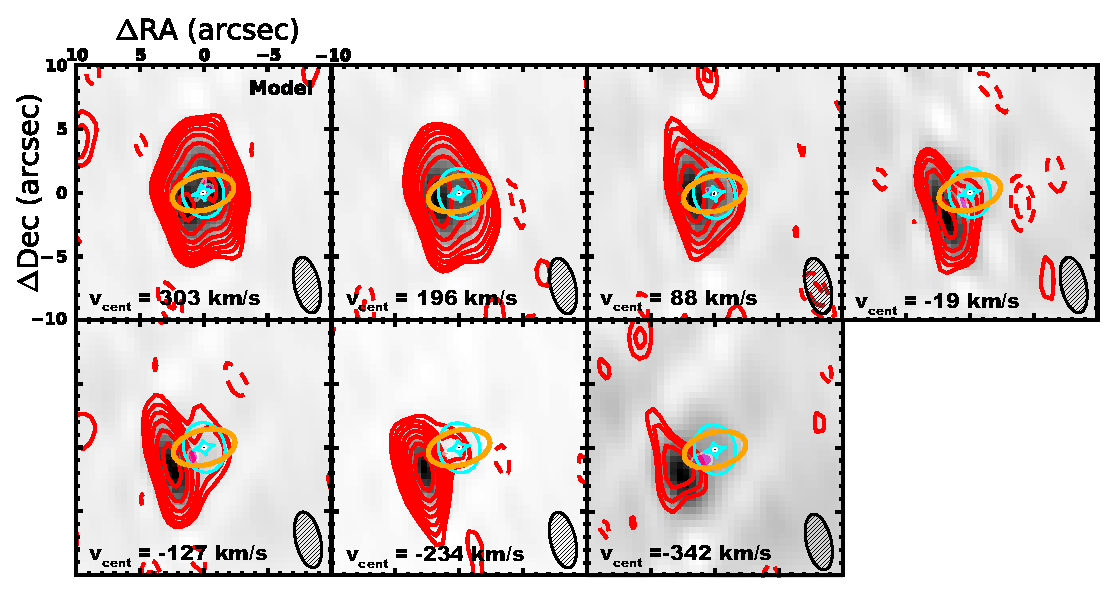
\includegraphics[width=0.85\textwidth]{../Figures/PostageStampModel.eps}
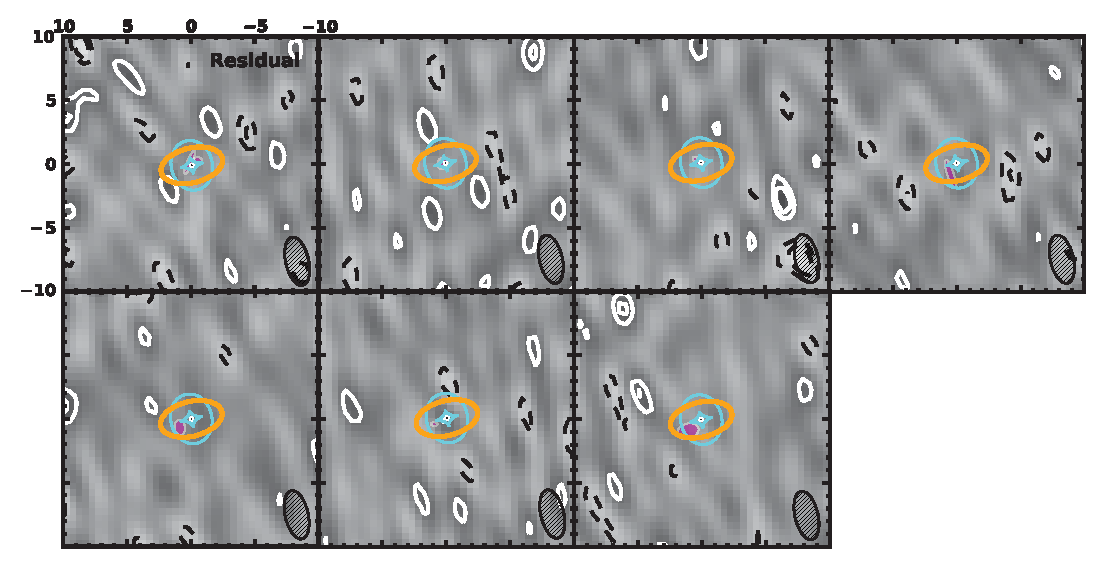
\includegraphics[width=0.85\textwidth]{../Figures/PostageStampResiduals.eps}
\caption{
Lens model of channel widths $\sim$ 100\kms.
Make this bigger in the future
Channel maps of the CO emission (red) overlaid on our best-fit lens models (grayscale). The foreground lensing galaxy is represented by a black dot. The reconstructed source morphology (magenta ellipses) is also suggestive of a “disk”.
\label{fig:model}}
\end{figure*}



\subsubsection{Differential Lensing} \label{sec:differential}
Lens modeling of this source from previous studies find non-negligible differential lensing effect across H-Band, V-band, and I-band. The magnification factor ranges from 10.9
to 7.8, where the decrease is caused
by the more extended IR emission (hence \SF), well beyond the caustic (C06).

The highly asymmetric \bco line profile also suggests that differential lensing is non-negligible in the CO emission, where
flux density in the red wing is apparently much higher than in the blue wing, given its lensing configuration.
By modeling different kinematic components, we find that the magnification factor ranges from BLAH to BLAH. The various magnification factors are listed in \Tab{mag}.
\begin{deluxetable}{lcc}[!htbp]
\tabletypesize{\scriptsize}
\tablecolumns{3}
\tablecaption{Magnification factors of various kinematic components in \bco}
\tablehead{
\colhead{Velocity Range(\kms)} & % see 22May16/intensity30Apr16.spec; or channel map in paper
\colhead{Source 1 $\mu_{\rm L}$} &
\colhead{Source 2 $\mu_{\rm L}$}
}
\startdata
$-$366\,$-$\,$-$258 & 3.1 $\pm$ 0.9 & \\ [0.5ex]
$-$237\,$-$\,$-$151 & 4.3 $\pm$ 2.4 & \\ [0.5ex]
$-$129\,$-$\,$-$43  & 4.2 $\pm$ 0.6 & \\ [0.5ex]
$-$21.5\,$-$\,65    & 4.1 $\pm$ 0.9 & \\ [0.5ex]
86\,$-$\,172        & 8.7 $\pm$ 2.0 & \\ [0.5ex]
194\,$-$\,280       & 7.6 $\pm$ 1.6 & \\ [0.5ex]
301\,$-$\,388       & 7.2 $\pm$ 5.6 & 6.7 $\pm$ 2.5 \\ [0.5ex]
weighted average & 4.4 & \\ [0.5ex]
median & 5.5 &
\enddata
\label{tab:model}
\tablecomments{Velocity is taken from the center of each (native) channel
without any binning. Each row corresponds to a channel slice used for
lens modeling. Source 1 is RXJ1131 and source 2 is its companion. See text for details. }
\end{deluxetable}




\subsection{\bco Dynamical modeling} \label{sec:dynamics}
Based on the the source plane position of each kinematic components from the
lens model, a clear symmetric velocity gradient is seen, which is suggestive of a rotating disk. Assuming the observed velocities of the respective channels
correspond to solely the tangential components (i.e. $\theta$ = 0), we extract
the major axis along the best-fit slice across these source plane positions,
which is along PA of 121\degr.
We attempt to characterize the molecular gas kinematics using an empirically motivated disk model (e.g. Courteau97, Peuch+08, Miller+11):
\begin{equation}
V = V_0 + \frac{2}{\pi} V_{\rm a} \arctan(\frac{R}{R_{\rm t}}),
\end{equation}
where $V$ is the observed velocity, $V_0$ is the velocity at dynamical center, $V_{\rm a}$ is the asymptotic velocity, and $R_{\rm t}$ is the ``turnover'' radius at which the rotation curve
becomes flat. We perform non-linear least square fitting using an orthogonal distance regression to find the best-fit $V_a$, $r_t$, $V_0$, taking into account
errors in both velocity and distance offset (see \Figure{PV}). We also place an upper limit on $r_t$ $<$ 15 kpc (Miller+11, Genzel+??, Puech+08?) to keep this
parameter physical. We then estimate the uncertainties associated with best-fit parameters using a Monte Carlo simulation of 500 iterations, perturbing
the velocity and physical separation according to a random Gaussian distribution of width/sigma based on the input uncertainties on
the data. Using this model, we find $V_a$ = 975$\pm$387, $r_t$ = 10.6$\pm$5.7,
and $V_0$ = 28$\pm$40. We note, however, that since emission is not detected beyond the flat regime of the rotation curve (Figure \ref{fig: PV}), the asymptotic velocity is
poorly constrained. In particular, $V_a$ and $r_t$ are highly correlated with a Pearson coefficient $r$ = 0.998 between the two, and 0.027 between $V_a$ and $V_0$.

While a symmetric velocity field in the source plane is consistent with a rotating disc, such is insufficient to conclude a rotating disk morphology. Additional characteristics such
as peak velocity dispersion at the center of a galaxy and a ``spider'' diagram are needed. Based on the reconstructed source plane in the optical/NIR emission, C06 find that a
n=1 Sersic profile is best fit their model or is it the reconstructed emission (TBD).

The frequently used V$_{\rm max}$ (maximum measured velocity) is not equivalent to the
asymptotic value, Va, a mathematical extrapolation and typically not reached in
the observed rotation curve. Estimates of Va can depend critically on how well
the central region and turn over of the rotation curve are constrained. For the
remaining analysis, we adopt the asymptotic limit as a proxy to the rotation
curve. We also note that typical studies of the Tully-Fisher relation uses V$_2.2$ (at 2.2 $\times$ disc scalelength $\sim$ 1.375 half-light radius $\sim$ 0.7R$_opt$) as the rotation
velocity since this would be the radius at which the velocity of a pure
exponential disc peaks at. However, our source appears to be a disturbed
rotator, albeit coarse resolution. Hence, rather than adopting V$_2.2$, we use the
asymptotic value from the best-fit arctangent model. The half light radius in the
optical is ~xx kpc (from C06; converted in to our cosmology, but BJB 8 kpc
across?).

If we adopt the best-fit parameters, we find a dynamical mass of $M_{\rm dyn}$($<$blah kpc) sin$^2 i$ = BLAH \Msun. Consider the line widths using the separation between
the red- and blue- shifted emission of the \bco line profile of $\Delta v_{\rm sep}/2 \sim$ blah \kms and a source size of blah kpc, we find a dynamical mass of $M_{\rm dyn}$
sin$^2 i$ = BLAH \Msun. If we adopt the inclination angle using the morphological axis ratio from the
reconstructed optical image reported by C06, where the minor axis is 1\farcs8 and the major axis is 3\farcs3.25, then we find an inclination angle of 56.4
\degr. Then $M_{\rm dyn}$\,=\,BLAH. The inclination angle is consistent with the observed unobscured AGN and an observable double peak line profile.

We note, however, that large differences (up to $\gtrsim$10 deg) can be found between such kinematically-derived inclinations and the ones inferred from the morphological
axis ratio (e.g., Chemin et al. 2006). We caution that this analysis is based on limited spatial resolution data and will been verified by future higher-resolution observations.

\subsection{SED modeling}
\subsection{ISM properties}
\subsection{Gas Mass}
\subsection{Source Extent}
Compared to HST:

%--------------------------------------------------------------------------
%                                Discussion
%--------------------------------------------------------------------------
\section{Discussion}
\subsection{Merger stage of RXJ1131-1231}



\subsection{Implications}
gas fraction at this redshift. how does that relate to
the SFH, and the change in cosmic SFD is due to change in gas content.
SFE at this redshift, how does that relate to the SFH. probably a secondary effect to the drop in SFH


%--------------------------------------------------------------------------
%                                Conclusions
%--------------------------------------------------------------------------
\section{Summary and Conclusions}
We studied a wet-wet merger between a AGN/starburst ULIRG and a optically faint companion at $z$ $\sim$ 0.65.
In this paper, we BLAH, refining the redshift to $z_{\rm CO}$=0.65370$\pm$0.0005.




%==============================================================================
%                                Back matters
%==============================================================================


% ACKNOWLEDGEMENTS
%-----------------
\acknowledgments


  %--------------------------------------------------------------------------
  %                               Bibliography
  %--------------------------------------------------------------------------
\bibliographystyle{yahapj}
\bibliography{RXJ.bib}
\end{document}